\documentclass[a4paper]{article}

\usepackage{graphicx}
\usepackage{amsmath,amssymb}
\usepackage{hyperref}
\usepackage{minted}
\usepackage{multirow}
\usepackage{comment}
\usepackage{float}
\usepackage{todonotes}

\title{Experimental setup}
\author{}
\date{}

\begin{document}
    \maketitle
    This part provides a template for describing the condition under which the experiment was done.
        
        \paragraph{Learning phases}
            Online telemetry recording
    
            offline transformer, cluster
            
            
            \begin{figure}[H]
                \centering
                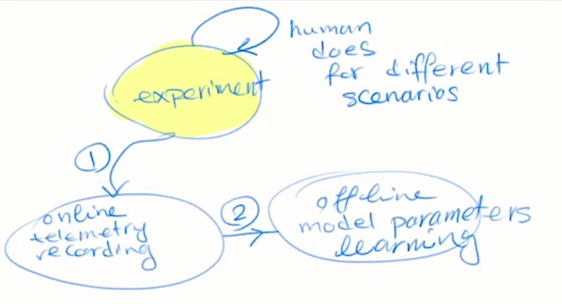
\includegraphics[width=0.9\textwidth]{learning_phases.png}
            \end{figure}
        \section{Goal}
            The goal is that two robots learn what it is like to turn around a square like corrider corrider without colliding the walls by human teleportation control and then
        \suction{Involving Robots}
            \subsubsection{MRS architecture}
                During online recording, a leader-follower strategy has been practiced by the two involving UAVs. The leader is the robot to which the human operator sends control inputs. The follower follows a set of rules which are dependent on leader's positional state.   during online telemetry recording, moves according to previously given ruls to update its position every $t$ \todo[inline]{find this in the code} seconds.
            \subsection{UAVs}
                Tarrot T650, Oldest
                
                
                
                
                
                
                
                \subsubsection{Sensors}
                    % to find frequencies, run /home/donkarlo/Dropbox/repo/nd_robotic_project/src/nd_robotic_ai/platform/ros/message/message_frequency_finder.py
                    
                    \paragraph{GPS}
                        \begin{itemize}
                            \item \textbf{Frequency:} 83.33 Hz
                        \end{itemize}
                    
                    \paragraph{LIDAR}
                        \begin{itemize}
                            \item \textbf{Frequency:} 20.83 Hz
                        \end{itemize}
    
            \subsection{Environment}
                The world is simulated by Gazebo and the robot simulation is done by ROS.
            
            \subsection{Human}
                Human is also considered as a
                
            \subsection{Homegeonity}
                Homogenous
            
            \subsection{Dependency}
                Leader-Followers
            
            
    
    
    \section{Condition}
        
        \subsection{Normal condition}
            \paragraph{Environment}
                A square corridor like the image below
            \paragraph{Maneuver}
                The two drones keep the same distance (Goal, keeping the same distance as much as possible while meeting everypoint on both  walls) while turning around the square corridor.
            \begin{figure}[H]
                \centering
                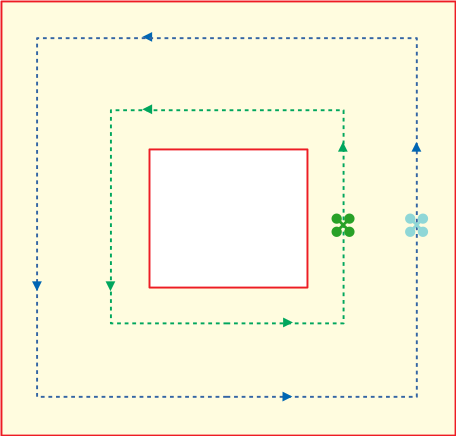
\includegraphics[width=0.9\textwidth]{normal.png}
            \end{figure}
        
        \subsection{Follow condition}
            On one side of the square corridor, the corridor becomes symmetrically narrower,\ref{} and consequently the human controller sends necessary commands to uav1
            \begin{figure}[H]
                \centering
                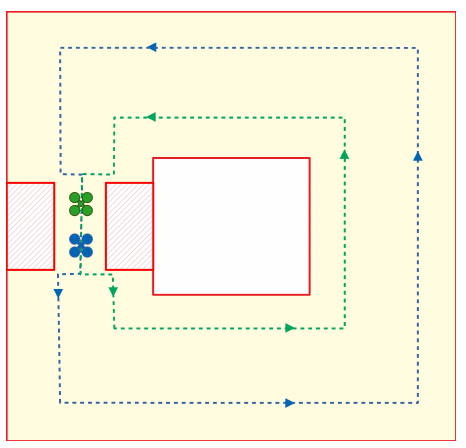
\includegraphics[width=0.9\textwidth]{follow.png}
                \label{follow}
            \end{figure}
        
        \subsection{Next to}
            \begin{figure}[H]
                \centering
                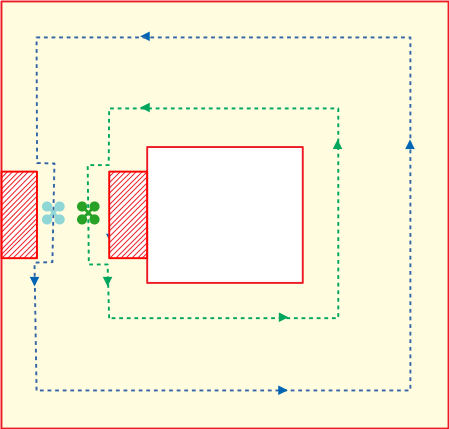
\includegraphics[width=0.9\textwidth]{next_to.png}
            \end{figure}

\end{document}